
\begin{algorithm}[!t]
\small
\caption{Label propagation algorithm}
\label{alg:SV_ALG}
\begin{algorithmic}[1]
\Require {$G=(V,E)$}

\State Initialization ;
\For {each $v\in V$}
\State	$CC[v]=v; CCp[v]=v$;
\EndFor

\State $NumChange=|V|$
\While{$NumChange>0$};
\State $NumChange\leftarrow 0$
\State MemCpy($CCp$,$CC$,$|V|$)
\For {each $v\in V$}
\For {each $u\in E(v)$}

\If {$CCp[u]<CC[v]$}
\State $CC[v]\leftarrow CCp[u]$
\State NumChanges = NumChanges+1;
\EndIf

\EndFor
\EndFor

\EndWhile 


\end{algorithmic}
\end{algorithm}
%

%intro to siloch-vishkin
We use Siloach and Vishkin algorithm (cite) for calculating connected component of
 the graph, as the baseline algorithm and modify the algorithm to make it fault tolerant.
 The!~\sv algorithm is based on so-called ``label-propagation'' techniques. 
 It is embarrassingly parallel, thus it can be efficiently implemented on highly concurrent
 shared memory (cite) and distributed memory architectures. 


 %description of the algorithm
 The~\sv algorithm is described in~\refalg{alg:SV_ALG}.
By convention, connected component id of any vertex is minimum vertex-id in its connected component.
  For all the vertices in the graph, 
 \sv algorithm maintains the current connected-component id array $CC$, which will contain 
 final connected component id at the end of computation. 

 In addition, to felicitate 
 concurrent execution, a connected component id from previous iteration is also stored in array $CCp$.
 In the beginning of computation, $CCp$ array for each vertex is initialized to its vertex id. 
 %
In each~\sv iteration, each vertex traverses its adjacency list, and 
 computes the  minimum component-id of all its neighbors and stores it in the $CC$ array. 
 Thus, eventually minimum component id propagates to all the vertices in the given connected component.
 %
 We keep track of number of changes in $CC$ array occur in any iteration. The~\sv algorithm terminates 
 when no vertex changes its component-id in an~\sv iteration. 

 %
 Each iteration requires $\mathcal{O}(|V|+|E|)$ computations, since
the algorithm accesses all vertices and their respective adjacencies.
The maximal length of propagation is limited by
the graph diameter $d$. As such, the total time complexity
of the algorithm is $\mathcal{O}(d.(V+E))$. Relative to~\refalg{alg:SV_ALG},
there is a shortcut that can reduce the number of iterations
to $d/2$. However, this does not change the asymptotic
time complexity of the algorithm, and we do not consider it
further

% insert figure here
Conceptually, the component labels propagate as~\reffig{fig:svPropagation}
depicts. Initially (a), four of the components have minimal
labels locally; these labels propagate gradually, and the label
of a given node may change several times, (b)-(e), possibly
even within the same iteration. Eventually, the algorithm
reaches a final state (e) where for a fully-connected graph
there will be a single connected component.



\begin{figure*}[t]
\centering
	\subfloat[]{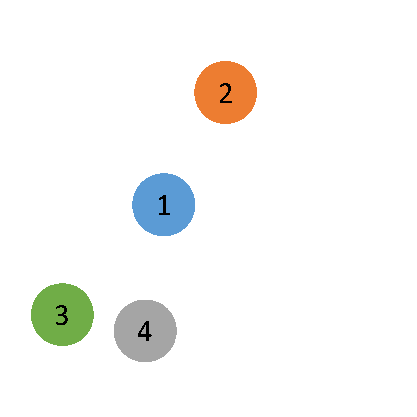
\includegraphics[width=0.2\textwidth]{figure/sv1.pdf}}
	\subfloat[]{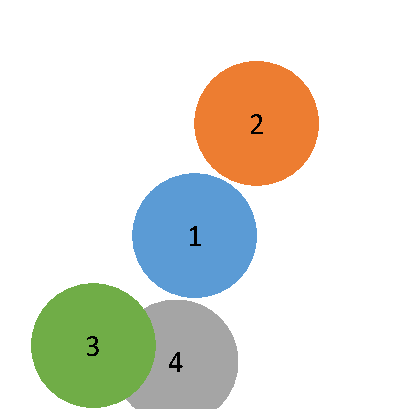
\includegraphics[width=0.2\textwidth]{figure/sv2.pdf}}
	\subfloat[]{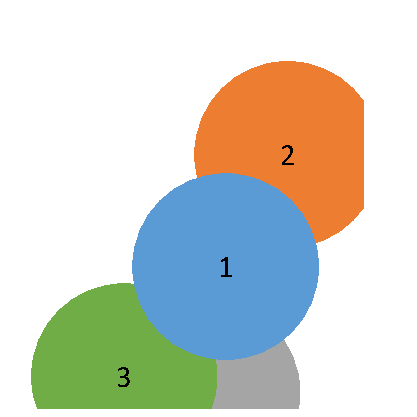
\includegraphics[width=0.2\textwidth]{figure/sv3.pdf}}
	\subfloat[]{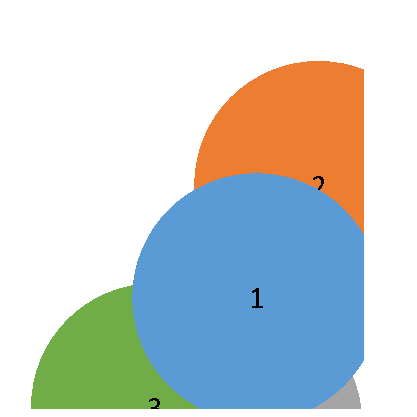
\includegraphics[width=0.2\textwidth]{figure/sv4.pdf}}
	\subfloat[]{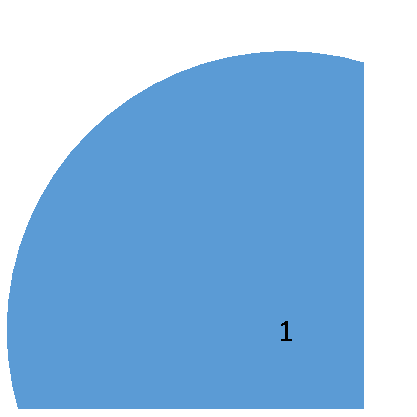
\includegraphics[width=0.2\textwidth]{figure/sv5.pdf}}

  \caption{These sub-figures conceptually show how the connected component id propagates through the graph as time evolves - each subfigure is for a different iteration of the algorithm. This example assumes that all vertices are connected and for simplicity shows only the connected components are 1 through 4. Initially the number of connected components is equal to the number vertices. (a) Depicts the initial state in which each vertex is in its own component. (b)-(d) depict that some vertices belong to the same connected component yet may require multiple label updates (in either the same iteration or a separate iteration).
	(e) is the final state in which there is a single connected component.}
  \label{fig:svPropagation}
\end{figure*}